\newprob{1715665463}
{
    下列哪一個證明了光是一種電磁波?\\
    \begin{itemize}
        \item[] (1) 當光穿過邊界從一種介質到另一種介質時,它會偏折。
        \item[] (2) 當光遇到一個光滑的表面時,它會反射。
        \item[] (3) 光可以從太陽到達地球。\\
    \end{itemize}
    \begin{choices}
        \choice 只有(1)
        \CorrectChoice 只有(3)
        \choice 只有(1) 和 (2)
        \choice 只有(2) 和 (3)
    \end{choices}
}{\mckey{B}}

\newprob{1715666244}
{
    一個繞射光柵每毫米有 500 條線,被白光垂直照射。如果黃光的波長為 600 nm,紫光的波長為 400 nm,以下哪些說法是正確的?\\

    \begin{itemize}
        \item[] (1) 在一階譜線中,紫色端比紅色端更靠近中央亮紋。
        \item[] (2) 黃光的二階像與紫光的三階像重合。
        \item[] (3) 紫光沒有四階像。\\
    \end{itemize}
    \begin{choices}
        \CorrectChoice 只有(1) 和 (2)
        \choice 只有(1) 和 (3)
        \choice 只有(2) 和 (3)
        \choice (1)、(2) 和 (3)
    \end{choices}
}{\mckey A}

\newprob{1715666262}
{
    在固定距離外,兩個相干波源產生了干涉圖案,以下那一個情況下腹線的間距是最長的?\\
    \begin{choices}
        \choice 相距5 mm的光源,波長為650 nm的紅光
        \choice 相距150 mm的點振源,並發出波長為5 mm的水波
        \choice 相距2 mm的光源,並發出波長為500 nm的藍光
        \CorrectChoice 相距45 mm的聲源,並發出波長為15 mm的聲波\\
    \end{choices}
}{\mckey D}

\newprob{1715666279}
{
    在楊氏雙縫實驗中,若狹縫間距過大,將有什 麼後果?

    \begin{enumerate}[label=\sd]
        \item 到達屏幕的光,強度將太弱,以致條紋不 易觀察。
              \par
        \item 條紋過於互相接近,以致條紋難於分辨。
              \par
        \item 光疊加時,不會產生相消干涉。
              \par
    \end{enumerate}


    \begin{choices}
        \choice 只有(1)
        \CorrectChoice 只有(2)
        \choice 只有(1)和(2)
        \choice 只有(2)和(3)
    \end{choices}

}{\mckey B}

\newprob{1715666289}
{
    上圖顯示,使用透射光柵來檢視一個單色光源。米尺放在1.5 m 外,且垂直於連接光源與光柵之間的直線。尺子讀數為``0"的位置緊貼這直線。現沿尺子移動一口針,直至針與光源的第1級像互相重疊。這時,尺子的讀數為 27.4 cm。若光柵每cm有3000條縫隙,光的波長是
    \begin{figure}[h!]
        \centering
        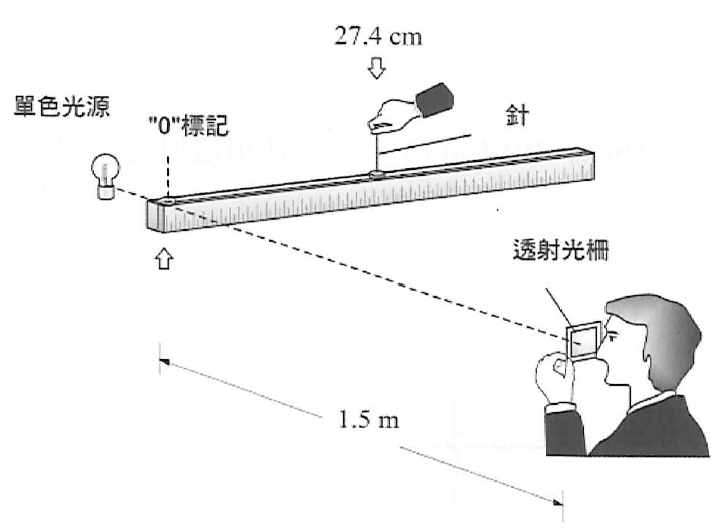
\includegraphics[width=.35\textwidth]{assets/80127820.png}
    \end{figure}
    \begin{choices}
        \choice \qty{4e-7}{m}
        \choice \qty{5e-7}{m}
        \CorrectChoice \qty{6e-7}{m}
        \choice \qty{7e-7}{m}
    \end{choices}

}{\mckey C}

\newprob{1715666306}
{
    在一個楊氏雙縫實驗中,使用波長為600 nm的單色光。縫隙之間的距離為0.06 mm。若總共觀察到十三條亮紋,這些條紋對向於雙縫中心所成的角$\theta$是多少?
    \begin{figure}[h!]
        \centering
        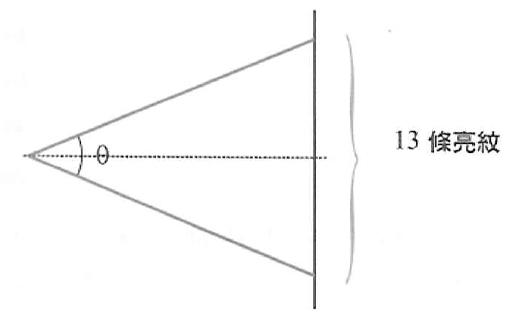
\includegraphics[width=.3\textwidth]{assets/b6bd221a.png}
    \end{figure}
    \begin{choices}
        \choice \qty{3.4}{\degree}
        \CorrectChoice \qty{6.9}{\degree}
        \choice \qty{7.5}{\degree}
        \choice \qty{15}{\degree}
    \end{choices}

}{\mckey B}

\newprob{1715666318}
{
    使用一組雙縫及波長為 \qty{7.0e-7}{m} 的紅光,以便產生干涉圖形。米尺放在雙縫外 1.5 m, 並垂直於連接雙縫與光源之間的直線。尺子上設有兩 個相距 0.20 m 的標記。標記之間共可 觀察到十三條亮紋,且每個標記均位於一個亮 紋的中央。縫隙的間距是多少?
    \begin{figure}[h!]
        \centering
        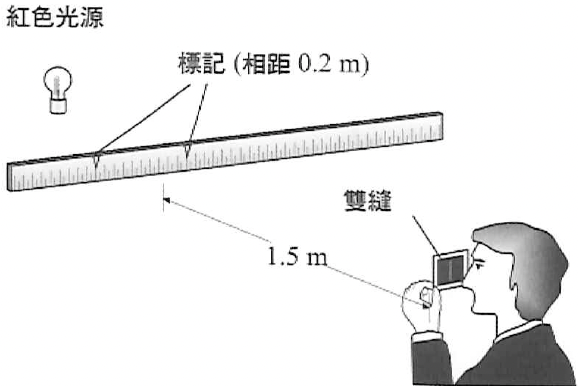
\includegraphics[width=.3\textwidth]{assets/2c8c3161.png}
    \end{figure}
    \begin{choices}
        \choice \qty{5.25e-5}{m}
        \CorrectChoice \qty{6.30e-5}{m}
        \choice \qty{1.05e-4}{m}
        \choice \qty{1.26e-4}{m}
    \end{choices}
}{\mckey B}

\newprob{1715666329}
{
    在一個楊氏雙縫實驗中,使用波長為600 nm 的光。來自狹縫X和Y的光,在屏幕上P點的 程差是 3300 nm。X和 Y均與O相隔同等的距 離。下列哪些陳述是正確的?
    \begin{figure}[h!]
        \centering
        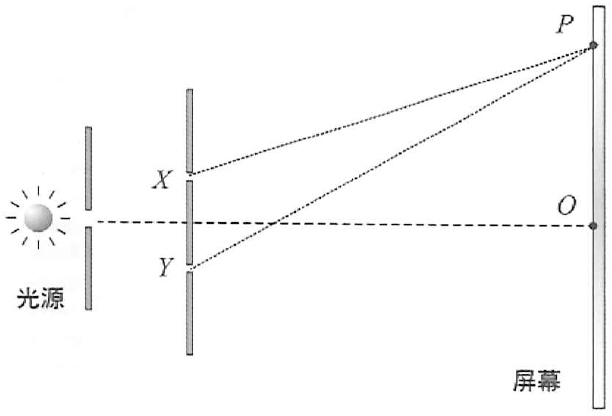
\includegraphics[width=.3\textwidth]{assets/e6bea960.png}
    \end{figure}

    \begin{statements}
        \task P位於一條暗紋之上。
        \task P和O之間共有六條暗紋,包括P和O上 的條紋。
        \task 若把光源移近狹縫,屏幕上條紋的間距 將會增加。
    \end{statements}



    \begin{choices}
        \CorrectChoice 只有(1)
        \choice 只有(2)
        \choice 只有(1)和(3)
        \choice 只有(2)和(3)
    \end{choices}

}{\mckey A}

\newprob{1715666342}
{
    兩個微波發射器P和 Q,面對面相距1 m,並 同時發出波長為3 cm 的微波。把一個探測器 從P移到Q時,首個強訊號出現在4點,而第 三個強訊號則出現在B點。A和B 之間相隔多 遠?
    \begin{center}

        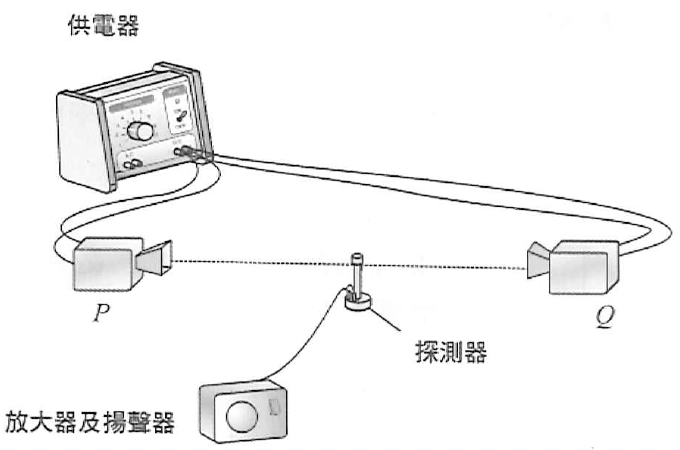
\includegraphics[width=.3\textwidth]{assets/158f4747.png}
    \end{center}
    \begin{choices}
        \choice 1.5 cm
        \choice 2 cm
        \CorrectChoice 3 cm
        \choice 4.5 cm
    \end{choices}

}{\mckey C}

\newprob{1715666360}
{
    金屬板放在一個產生波長為3 cm 的微波發射 器前。沿著XY 移動一個探測器,依次接收到 強弱交替的訊號。以下哪些數據可能是兩個相 鄰強訊號之間的距離?
    \begin{figure}[h!]
        \centering
        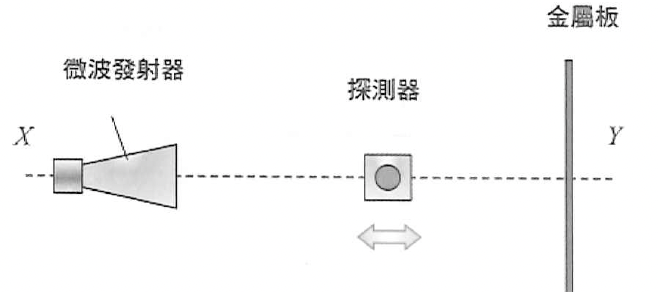
\includegraphics[width=.35\textwidth]{assets/e9d4c633.png}
    \end{figure}

    \begin{enumerate}[label=\sd]
        \item 1.5 cm
              \par
        \item 3 cm
              \par
        \item 4 cm
              \par
    \end{enumerate}


    \begin{choices}
        \choice 只有(2)
        \CorrectChoice 只有(1)和(2)
        \choice 只有(2)和(3)
        \choice (1)、(2)和(3)
    \end{choices}

}{\mckey B}